\chapter{Interfacce}

Per realizzare le pagine sono stati usati \emph{HTML 5} e \emph{bootstrap} per definire la struttura 
degli elementi della pagina.\\ 
Gli elementi di personalizzazione, come il nome utente nella navbar una volta autenticati o il meteo 
in tempo reale delle città salvate tra i preferiti, sono inseriti utilizzando \emph{EJS}.

\vspace{5mm}

In ogni pagina, il contenuto del tag \emph{head} e alcuni script (necessari per dark mode toggle, bootstrap e 
ricerca di una città) sono aggiunti tramite l'utilizzo di \emph{partials}, elementi supportati da EJS.

\section{Index.ejs}

\begin{figure}[ht]
    \centering
    \resizebox{\textwidth}{!}{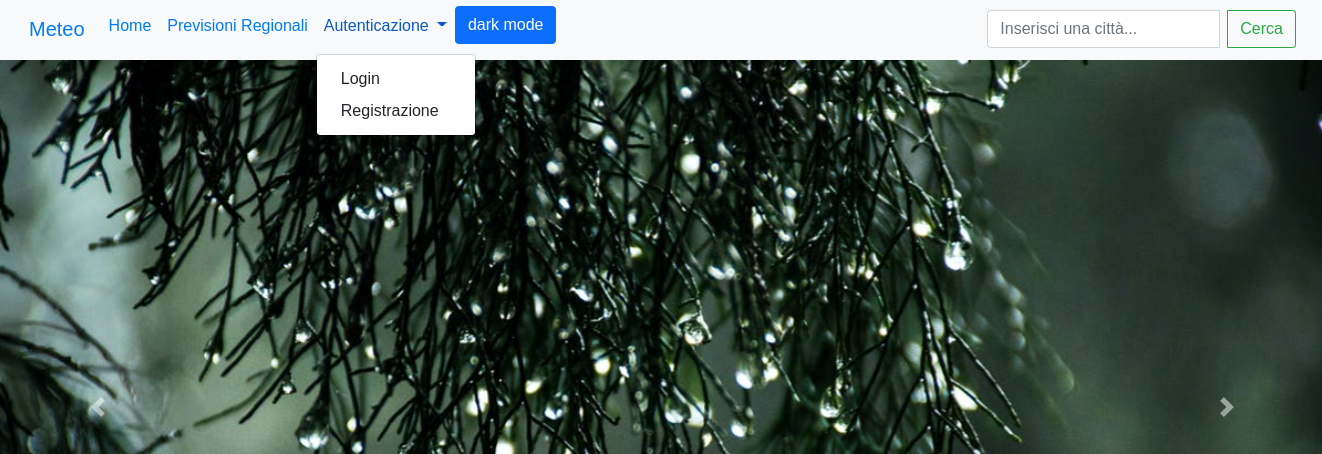
\includegraphics{img/indexSopra.png}}
    \caption{Metà superiore dell'home page}
\end{figure}

Nella metà superiore dell'index troviamo una navbar semplice ed intuitiva: abbiamo infatti la 
possibilità di vedere le previsioni delle province di ogni regione cliccando su 
\emph{Previsioni Regionali}, di autenticarci facendo il login o la registrazione tramite il menù a 
tendina apribile cliccando su \emph{Autenticazione} (menù che sarà sostituita con un altro  
a seguito del login per poter effettuare il logut e accedere all'area personale), di cambiare la visualizzazione 
della pagina dalla modalità \emph{dark mode} a quella \emph{light mode} ed infine di cercare una città tramite 
l'apposita barra di ricerca in alto a destra.\\
Al di sotto della navbar, troviamo uno slider temporizzato che mostra immagini relative a condizioni 
climatiche differenti. 

\newpage
\begin{figure}[ht]
    \centering
    \resizebox{\textwidth}{!}{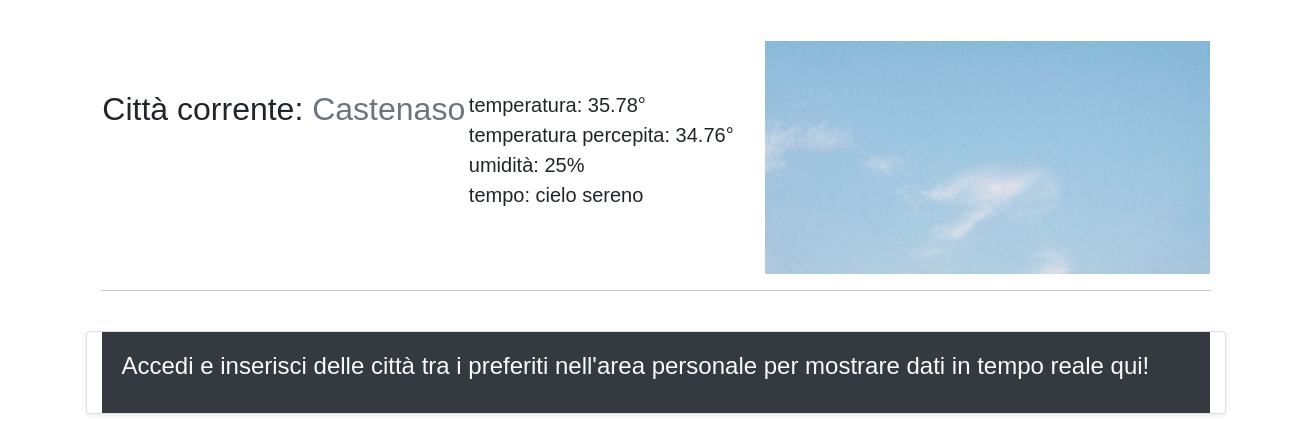
\includegraphics{img/indexSotto.png}}
    \caption{Metà inferiore dell'home page}
\end{figure}

Superato lo slider, troviamo una sezione dedicata alle condizioni meteo della città in cui ci troviamo 
(le coordinate sono ottenute con l'oggetto \emph{navigator.geolocation}, motivo per cui utilizzare una 
connessione da telefono cellulare garantirà una maggiore precisione) a seguito della quale è presente 
un'area dedicata alla visualizzazione delle città salvate tra i preferiti nell'area personale accessibile 
dopo il login.

\begin{figure}[ht]
    \centering
    \resizebox{\textwidth}{!}{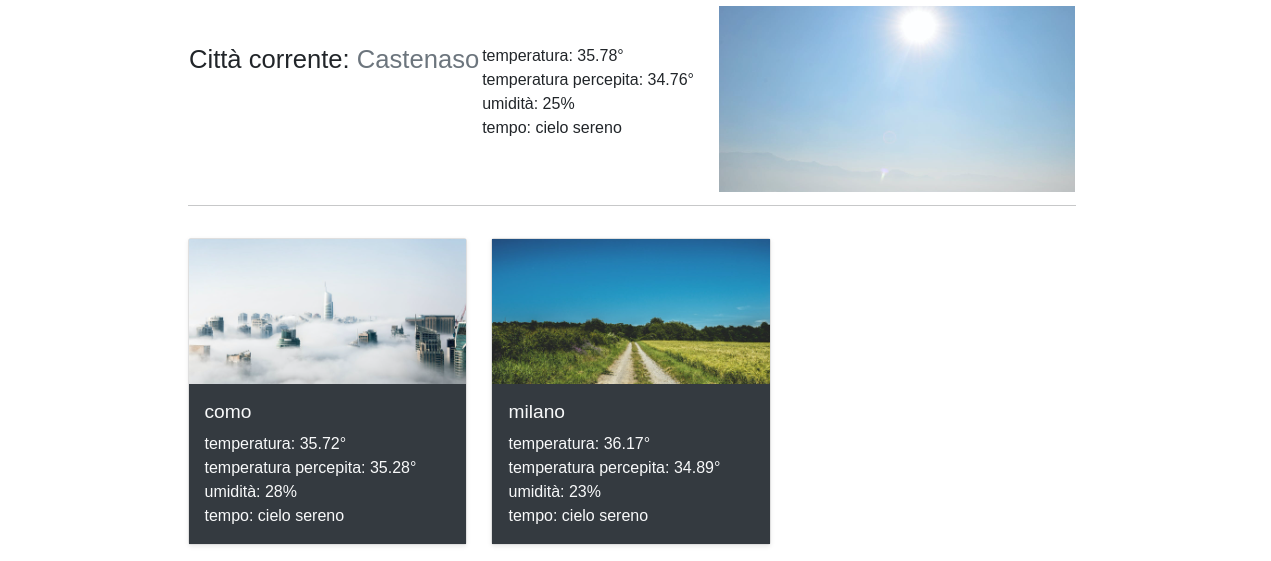
\includegraphics{img/indexLogged.png}}
    \caption{Metà inferiore dell'home page dopo aver effettuato il login}
\end{figure}

\newpage
\section{Previsioni}

\subsection{Regionali.ejs}

\begin{figure}[ht]
    \centering
    \resizebox{\textwidth}{!}{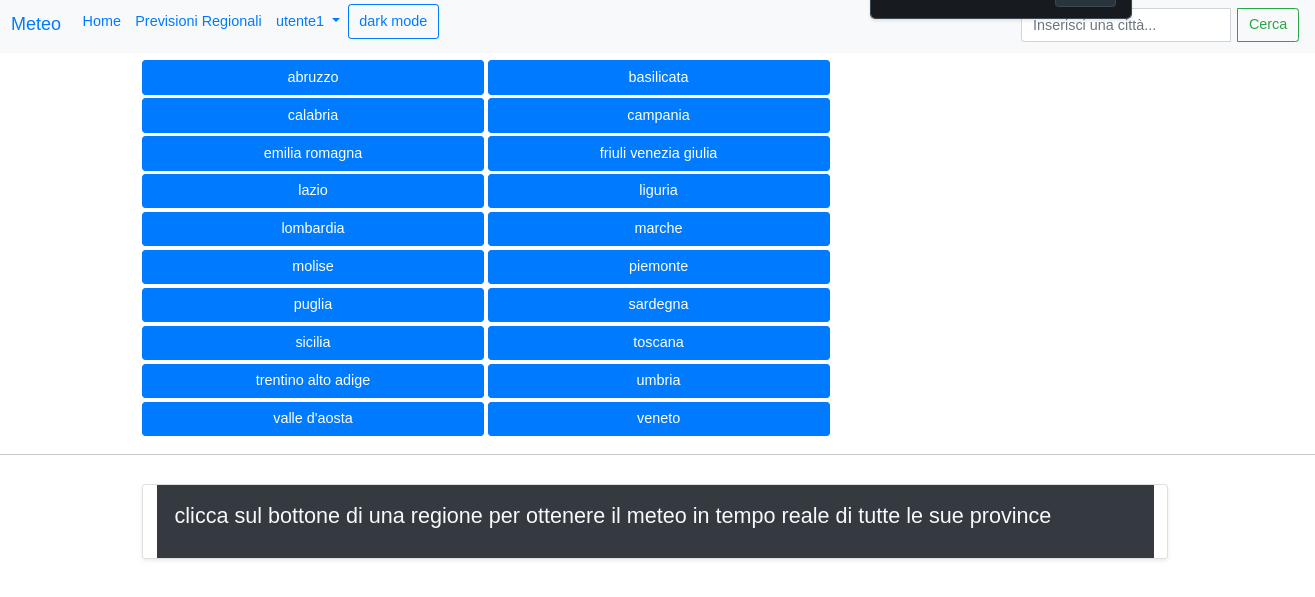
\includegraphics{img/previsioniRegionali.png}}
    \caption{Pagina dedicata alle previsioni regionali prima di cliccare su una regione}
\end{figure}

In questa pagina è possibile visualizzare le previsioni relative a tutte le province di una regione 
premendo sul tasto della regione voluta.\\
Fatto ciò, verrà visualizzato per ogni provincia un riquadro analogo a quelli presenti nell'index dopo 
il login con le informazioni metereologiche in tempo reale.

\begin{figure}[ht]
    \centering
    \resizebox{\textwidth}{!}{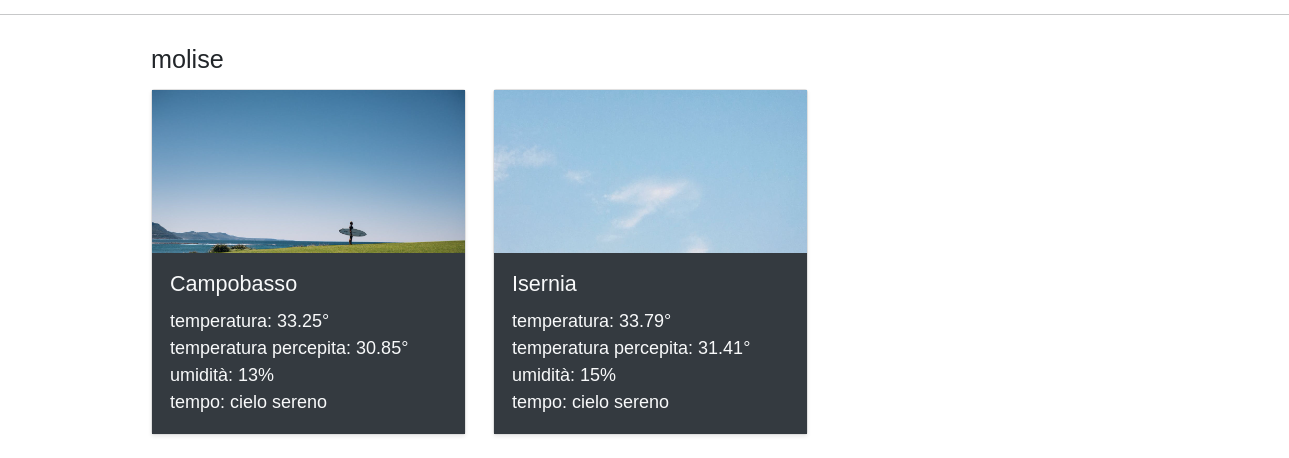
\includegraphics{img/previsioniRegionaliMolise.png}}
    \caption{Nell'immagine di esempio, la regione selezionata è stata il Molise}
\end{figure}

\newpage
\subsection{CitCercata.ejs}

\begin{figure}[ht]
    \centering
    \resizebox{\textwidth}{!}{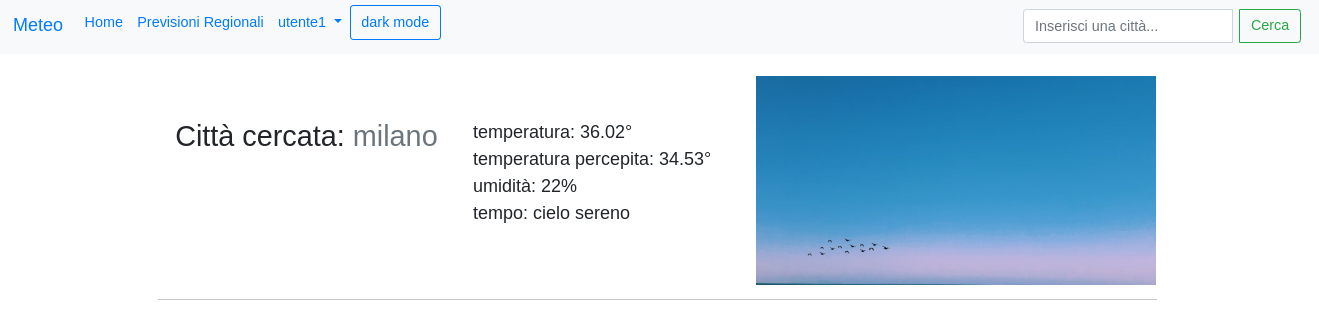
\includegraphics{img/citCercata.png}}
    \caption{Pagina visualizzata a seguito della ricerca di una città nella navbar}
\end{figure}

Attraverso la barra di ricerca in alto a destra nella navbar, è possibile cercare il nome della città per cui si 
vogliono ottenre le condzioni meteo in tempo reale.\\

\vspace{5mm}

Scrivendo il nome, verrà visualizzato a sinistra dell'input una scritta che informerà l'utente se lacittà inserita 
risulta esistente o meno (il sistema è strutturato per non essere \emph{case sensitive}). Nel caso in cui la città risulti 
esistente, verrà visualizzata la pagina in immagine, in caso contrario si rimarrà sulla pagina da cui si aveva fatto la ricerca.

\section{Login e Registrazione}

\subsection{Login.ejs}

\begin{figure}[ht]
    \centering
    \resizebox{\textwidth}{!}{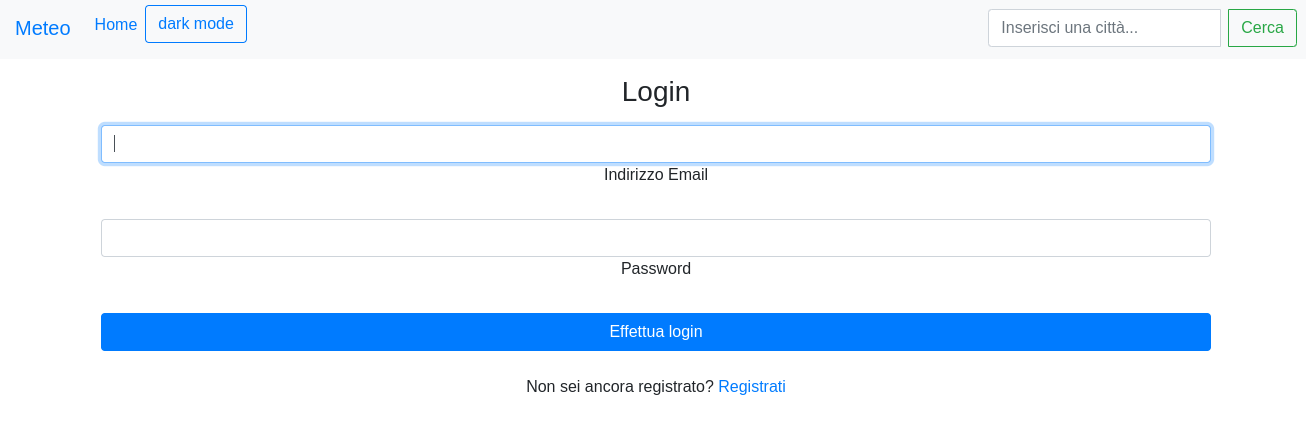
\includegraphics{img/login.png}}
    \caption{Pagina dedicata al login}
\end{figure}

Grazie a quest apagina è possibile effettuare il login nel caso si sia già registrati oppure di registrarsi attravero l'apposito 
link al di sotto del form con le credenziali.\\
La navbar è semplificata in modo da rendere l'interfaccia meno dispersiva e permette unicamente di tornare alla home, gestire 
la modalità di visualizzazione della pagina oppure cercare una città.

\newpage
\subsection{Registrazione.ejs}

\begin{figure}[ht]
    \centering
    \resizebox{\textwidth}{!}{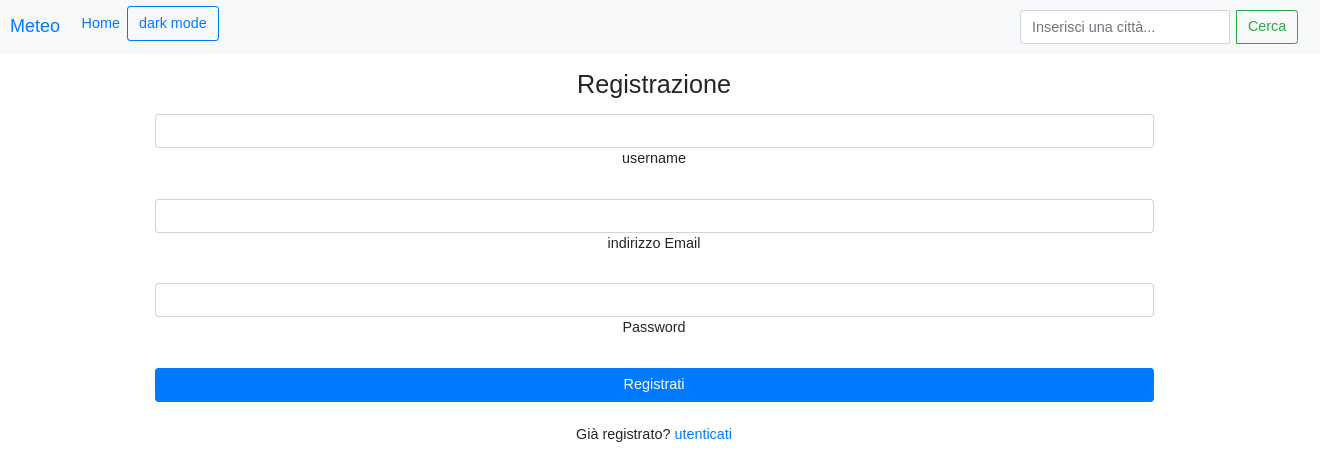
\includegraphics{img/registrazione.png}}
    \caption{Pagina dedicata alla registrazione}
\end{figure}

In questa pagina verranno richieste le credenziali usate in seguito per effettuare il login (email e password) e un nome utente. 
Questi dati saranno modificabili in un secondo momento tramite l'area personale (\textbf{N.B.}: non è possibile avere più utenti con 
la stessa mail e/o lo stesso username).\\

\vspace{5mm}

Se necessario, è possibile passare alla pagina di login tramite il link in basso.\\

\vspace{5mm}

La navbar è semplificata nella stessa maniera della pagina di login.

\subsection{AreaPersonale.ejs}

\begin{figure}[ht]
    \centering
    \resizebox{\textwidth}{!}{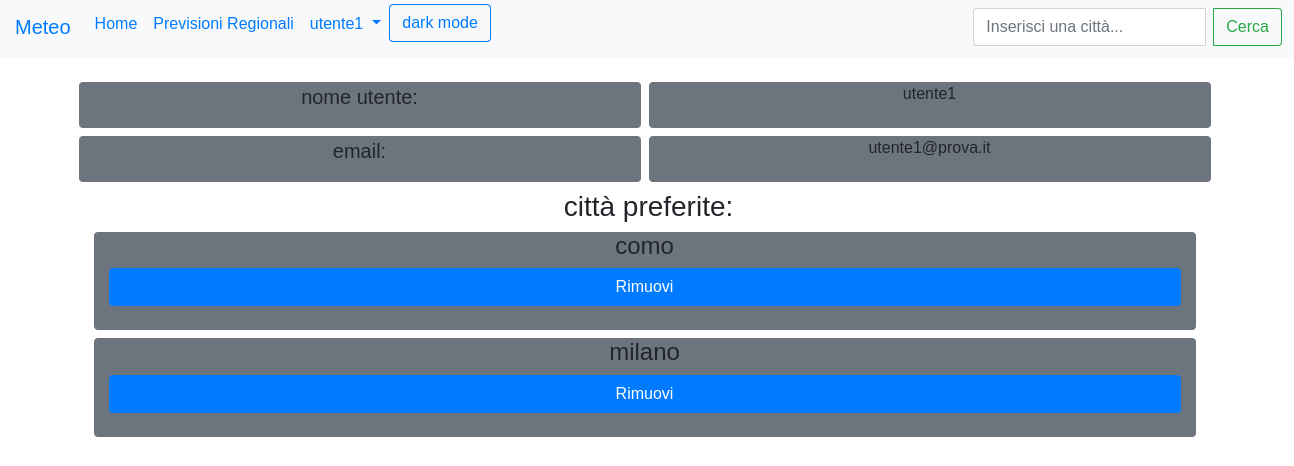
\includegraphics{img/areaPSopra.png}}
    \caption{Metà superiore della pagina dedicata all'area personale}
\end{figure}

Nella metà superiore della pagina troviamo una navbar analoga a quella presente nell'index a seguito del login.

\vspace{5mm}

Al di sotto di essa, abbiamo i dati relativi all'utente (username e email. la password non viene mostrata per ragioni di 
sicurezza) e l'elenco delle città salvate tra i preferiti, se presenti.

\begin{figure}[ht]
    \centering
    \resizebox{\textwidth}{!}{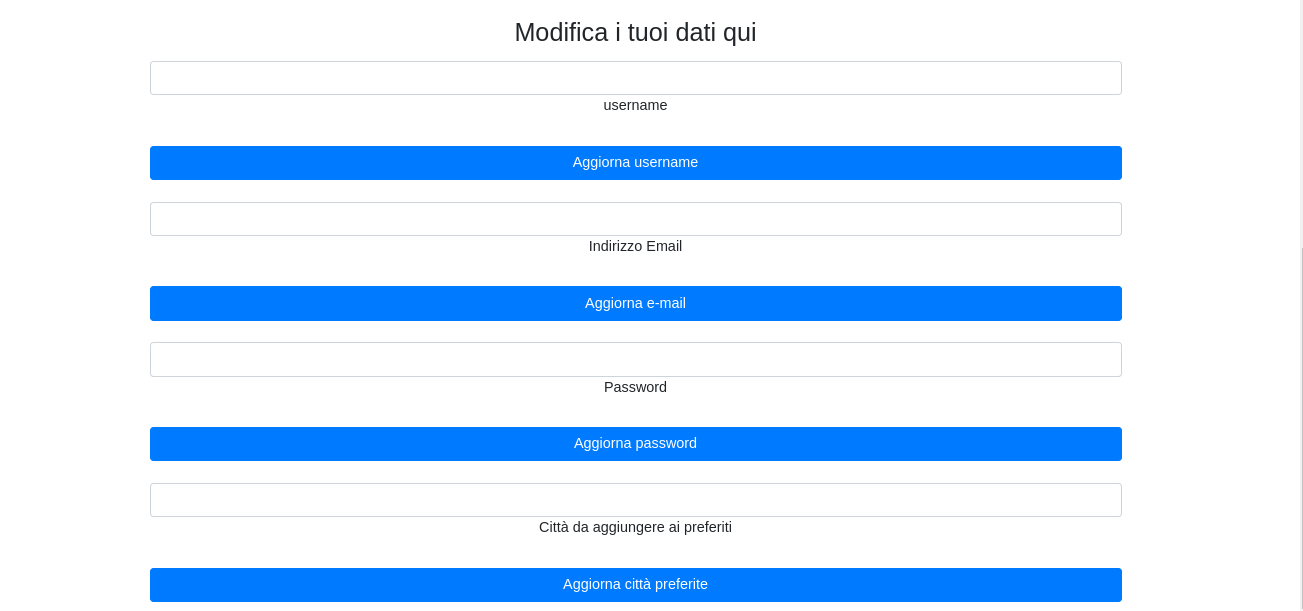
\includegraphics{img/areaPSotto.png}}
    \caption{Metà inferiore della pagina dedicata all'area personale}
\end{figure}

A seguito di queste informazioni, troviamo una serie di form che permettono, attraverso chiamate asincrone al server, di modificare 
i dati relativi all'utente, quali:
\begin{itemize}
    \item username
    \item email
    \item password 
    \item città salvate tra i preferiti
\end{itemize}